\documentclass[a4paper]{article}
\usepackage{fullpage}
\usepackage{graphicx}
\usepackage{xcolor}

\IfFileExists{.git/gitHeadInfo.gin}{
    \usepackage[pcount,grumpy,mark,markifdirty]{gitinfo2}
}{%
    \usepackage[local,pcount,grumpy,mark,markifdirty]{gitinfo2}
}



\usepackage{minted}
\usepackage{natbib}

\usepackage{hyperref}

\title{Template Repository for Articles}
\author{Christophe Prud'homme\thanks{Cemosis, IRMA UMR 7501, Université de Strasbourg, CNRS, France, \tt \href{mailto:christophe.prudhomme@cemosis.fr}{christophe.prudhomme@cemosis.fr}}}
\date{\gitReln\  \gitAuthorDate\ (\gitAbbrevHash)}

% Define custom color
\definecolor{CustomBlue}{rgb}{0.25, 0.41, 0.88} % RoyalBlue
% Set up hyperref with the custom citecolor
\hypersetup{
    pdftitle={\@title},
    pdfauthor={\@author},
    pdfsubject={\@subject},
    pdfkeywords={LaTeX, GitHub Actions, Zotero, Overleaf},
    bookmarksnumbered,bookmarksopen,linktocpage,
    colorlinks=true,
    citecolor=CustomBlue,
    linkcolor=CustomBlue,
    urlcolor=blue
}

% Define colors
\definecolor{background}{RGB}{245,245,244}
\definecolor{string}{RGB}{163,21,21}
\definecolor{keyword}{RGB}{0,0,255}
\definecolor{comment}{RGB}{0,128,0}
\definecolor{identifier}{RGB}{0,0,0}
\definecolor{bashkeyword}{RGB}{0,0,128}

% Minted settings
\setminted{
    bgcolor=background,
    fontsize=\footnotesize,
    linenos,
    breaklines,
    frame=single,
    framesep=2mm,
    tabsize=2
}

\begin{document}

\maketitle
\tableofcontents

\section{Introduction}
\label{sec:introduction}

Writing scientific articles using LaTeX offers numerous advantages, including precise typesetting, seamless integration of references, and robust version control. 
This template repository demonstrates best practices for organizing LaTeX projects, utilizing GitHub Actions for automated document compilation, managing bibliographies with Zotero, and optimizing image handling. 
By following this template, researchers can enhance their workflow efficiency and ensure consistent document formatting across platforms like Overleaf and local LaTeX installations.
The releases assets produced by the GitHub Actions allows to upload the article to HAL, arXiv, Zenodo, etc.



\section{Git Support}
\label{sec:git-support}

The `gitinfo2` package~\citep{brent_longborough_gitinfo2sty_2015} allows LaTeX documents to include information about the current state of the Git repository, such as the commit hash, author, and date. This is particularly useful for versioning and tracking changes in scientific documents.

\subsection{Configuration}

To include `gitinfo2` in your LaTeX document, add the following lines to your preamble:

\begin{minted}[bgcolor=background]{latex}
\IfFileExists{.git/gitHeadInfo.gin}{
    \usepackage[pcount,grumpy,mark,markifdirty]{gitinfo2}
}{%
    \usepackage[local,pcount,grumpy,mark,markifdirty]{gitinfo2}
}
\end{minted}

This configuration attempts to use .git/gitHeadInfo.gin if it exists (indicating a Git repository) and falls back to a local file if not.

\subsection{Setting Up Git Hooks}

To automatically generate the \mintinline{sh}|.git/gitHeadInfo.gin| file with each commit, you need to set up Git hooks. 
This repository includes a script \mintinline{sh}|setup-hooks.sh| to simplify the installation of these hooks.

\inputminted[linenos,autogobble,bgcolor=background,fontsize=\small]{sh}{setup-hooks.sh}

This will copy the \mintinline{sh}|post-commit| and \mintinline{sh}|post-checkout| hook scripts to the .git/hooks directory and make them executable. 
These hooks will automatically generate the \mintinline{sh}|.git/gitHeadInfo.gin| and update \mintinline{sh}|gitHeadLocal.gin| file after each commit or checkout.

The file \mintinline{sh}|gitHeadLocal.gin| is used when the document is compiled outside of a Git repository, e.g., in Overleaf or in an public archive such as HAL or arXiv.


\subsection{Using GitHub Actions}

The GitHub Actions workflow is configured to run the \mintinline{sh}|setup-hooks.sh| script, ensuring that the Git hooks are set up in the CI environment.
This allows the automated compilation of the LaTeX document to include the latest Git information in the article.

The template article repository workflow uses \citep{cheng_xu_xu-chenglatex-action_2024} \mintinline{bash}{xu-cheng/latex-action} to build the latex document.

The GitHub Action workflow:
\begin{itemize}
    \item Compiles the LaTeX document using \mintinline{bash}{xu-cheng/latex-action} on \texttt{ubuntu-latest} runner or \texttt{self-texlive} runner hosted on \texttt{feelpp} organisation.
    \item Uploads the resulting PDF
    \item Creates a release with the PDF as an asset when a new tag is pushed of the type \texttt{v*}, e.g., \texttt{v1.0.0}.
\end{itemize}

\subsection{Full Article Workflow}
\label{sec:full-article-workflow}


Here is a summary of the full workflow for creating and maintaining a LaTeX document with Git support:

\begin{enumerate}
    \item \textbf{Check out the organisation}: if the organisation is \texttt{feelpp} and a \texttt{self-texlive} labelled runner is online, the compilation will be done using the \texttt{self-texlive} runner other it will use the \texttt{ubuntu-latest} runner.
    \item \textbf{Clone the Repository}:
    Clone the repository to your local machine:
    \begin{minted}[bgcolor=background]{sh}
    git clone https://github.com/your-username/your-repo.git
    cd your-repo
    \end{minted}
    \item \textbf{Set Up Git Hooks}:
    Run the setup-hooks.sh script to set up the necessary Git hooks:
    \begin{minted}[bgcolor=background]{sh}
    ./setup-hooks.sh
    \end{minted}
    \item  \textbf{Compile the Document}:
    Compile the LaTeX document to generate the PDF:
    \begin{minted}[bgcolor=background]{sh}
    pdflatex -shell-escape main.tex
    \end{minted}
    \item \textbf{Make Changes to Your Document}:
    Edit your LaTeX document and add, commit, and push changes to the repository:
    \begin{minted}[bgcolor=background]{sh}
    git add .
    git commit -m “Update document”
    git push origin main
    \end{minted}
    \item \textbf{Create a Tag for Release}:
    Create and push a tag, using semver\footnote{\url{https://semver.org}},  to trigger the GitHub Actions workflow for building and releasing the document:
    \begin{minted}[bgcolor=background]{sh}
    ./release create v1.0.0
    \end{minted}
    \item \textbf{Review GitHub Actions Workflow}:
    The GitHub Actions workflow will automatically compile your LaTeX document and upload the resulting PDF as an artifact. 
    You can download the compiled PDF from the Actions tab in your repository.
    \item \textbf{Sync with Overleaf}:
    If you are using Overleaf, sync your GitHub repository with Overleaf to ensure you always have the latest version of your document.
\end{enumerate}

By following this workflow, you can efficiently manage your LaTeX documents, keep track of changes with Git, and automate the compilation and release process with GitHub Actions.

\subsection{Document Release}

The `release` script simplifies creating and listing releases for your LaTeX document. 

\inputminted[linenos, fontsize=\small, bgcolor=background]{sh}{release}



\begin{description}
    \item[Create a New Release]: To create a new release on GitHub, use the following command:
    \begin{minted}[bgcolor=background]{sh}
        ./release create v1.0.0
    \end{minted}
    \item[List All Releases]: To list all releases, use the following command:
    \begin{minted}[bgcolor=background]{sh}
        ./release list
    \end{minted}
    \item[Delete a Release]: To delete a release, use the following command:
    \begin{minted}[bgcolor=background]{sh}
        ./release delete v1.0.0
    \end{minted}

\end{description}

This script provides an easy interface for managing releases, automating the tagging, updating, committing, and pushing processes.


\section{Image Naming Convention}

To ensure compatibility with platforms like HAL, arXiv, and Overleaf, name your images with the \texttt{img-*} prefix and store them in the same directory as the \texttt{.tex} file. 
This makes it easier to manage and upload your images along with your LaTeX document.

\textbf{Example}:
\begin{itemize}
    \item \texttt{img-figure1.pdf}
    \item \texttt{img-figure2.png}
    \item \texttt{img-figure3.jpg}
\end{itemize}

\section{Using References from Zotero via Overleaf}

To manage your references with Zotero and integrate them seamlessly into Overleaf, follow these steps:

\subsection{Export Zotero Library to BibTeX}
\begin{enumerate}
    \item Open Zotero and select the references you want to export.
    \item Go to \texttt{File > Export Library}.
    \item Choose \texttt{BibTeX} as the format and save the file (e.g., \texttt{references.bib}).
\end{enumerate}

\subsection{Upload BibTeX File to Overleaf}
\begin{enumerate}
    \item Open your project in Overleaf.
    \item Click on the \texttt{Upload} button (top-left corner) and upload your \texttt{references.bib} file.
\end{enumerate}

\subsection{Include the Bibliography in Your LaTeX Document}

Add the following lines to your \texttt{.tex} file to include the bibliography:

\begin{minted}[bgcolor=background]{latex}
\documentclass{article}
\usepackage{graphicx}
\usepackage{natbib}
\begin{document}

% Your content here

\bibliographystyle{plainnat}
\bibliography{references}

\end{document}
\end{minted}

\subsection{Cite References in Your LaTeX Document}

Use the \mintinline{latex}{\cite} command to cite references within your document. For example:

\begin{minted}[bgcolor=background]{latex}
As shown by \citet{AuthorYear}, this method is effective.
\end{minted}



\section{Steps to Use the Template Repository}

\subsection{Create a New Repository}
Use the git template repository feature to create a new repository based on this template.

\begin{figure}[h!]
\centering
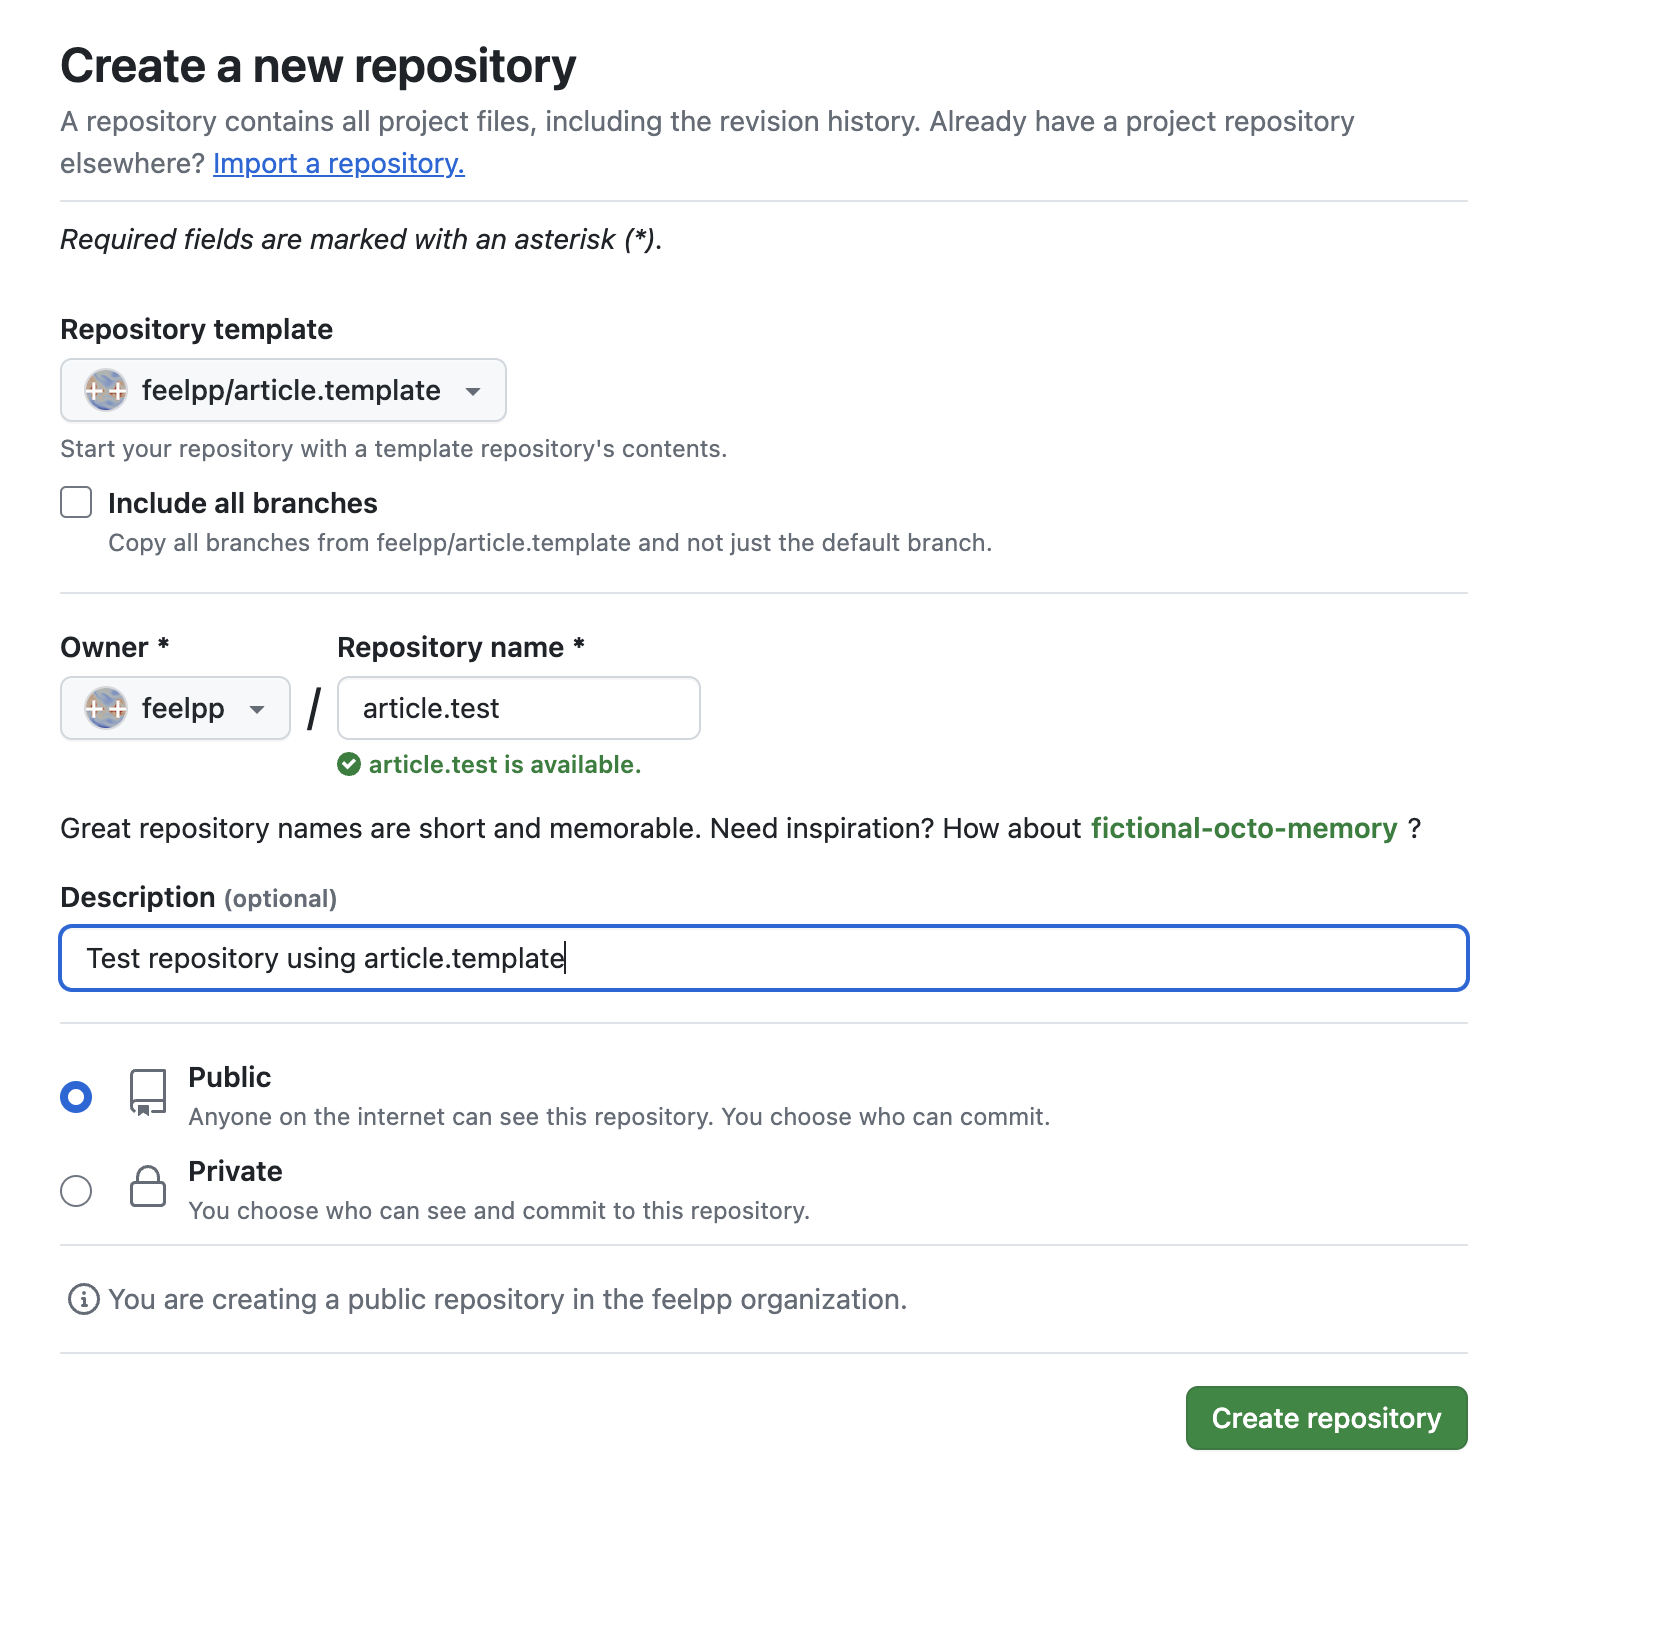
\includegraphics[width=0.8\textwidth]{img-create-repo.png}
\caption{Create a New Repository}
\end{figure}

\subsection{Clone the Repository}
Clone the repository to your local machine.

\begin{minted}[bgcolor=background]{bash}
git clone https://github.com/feelpp/my-repo.git
cd my-repo
\end{minted}

\begin{figure}[h!]
\centering
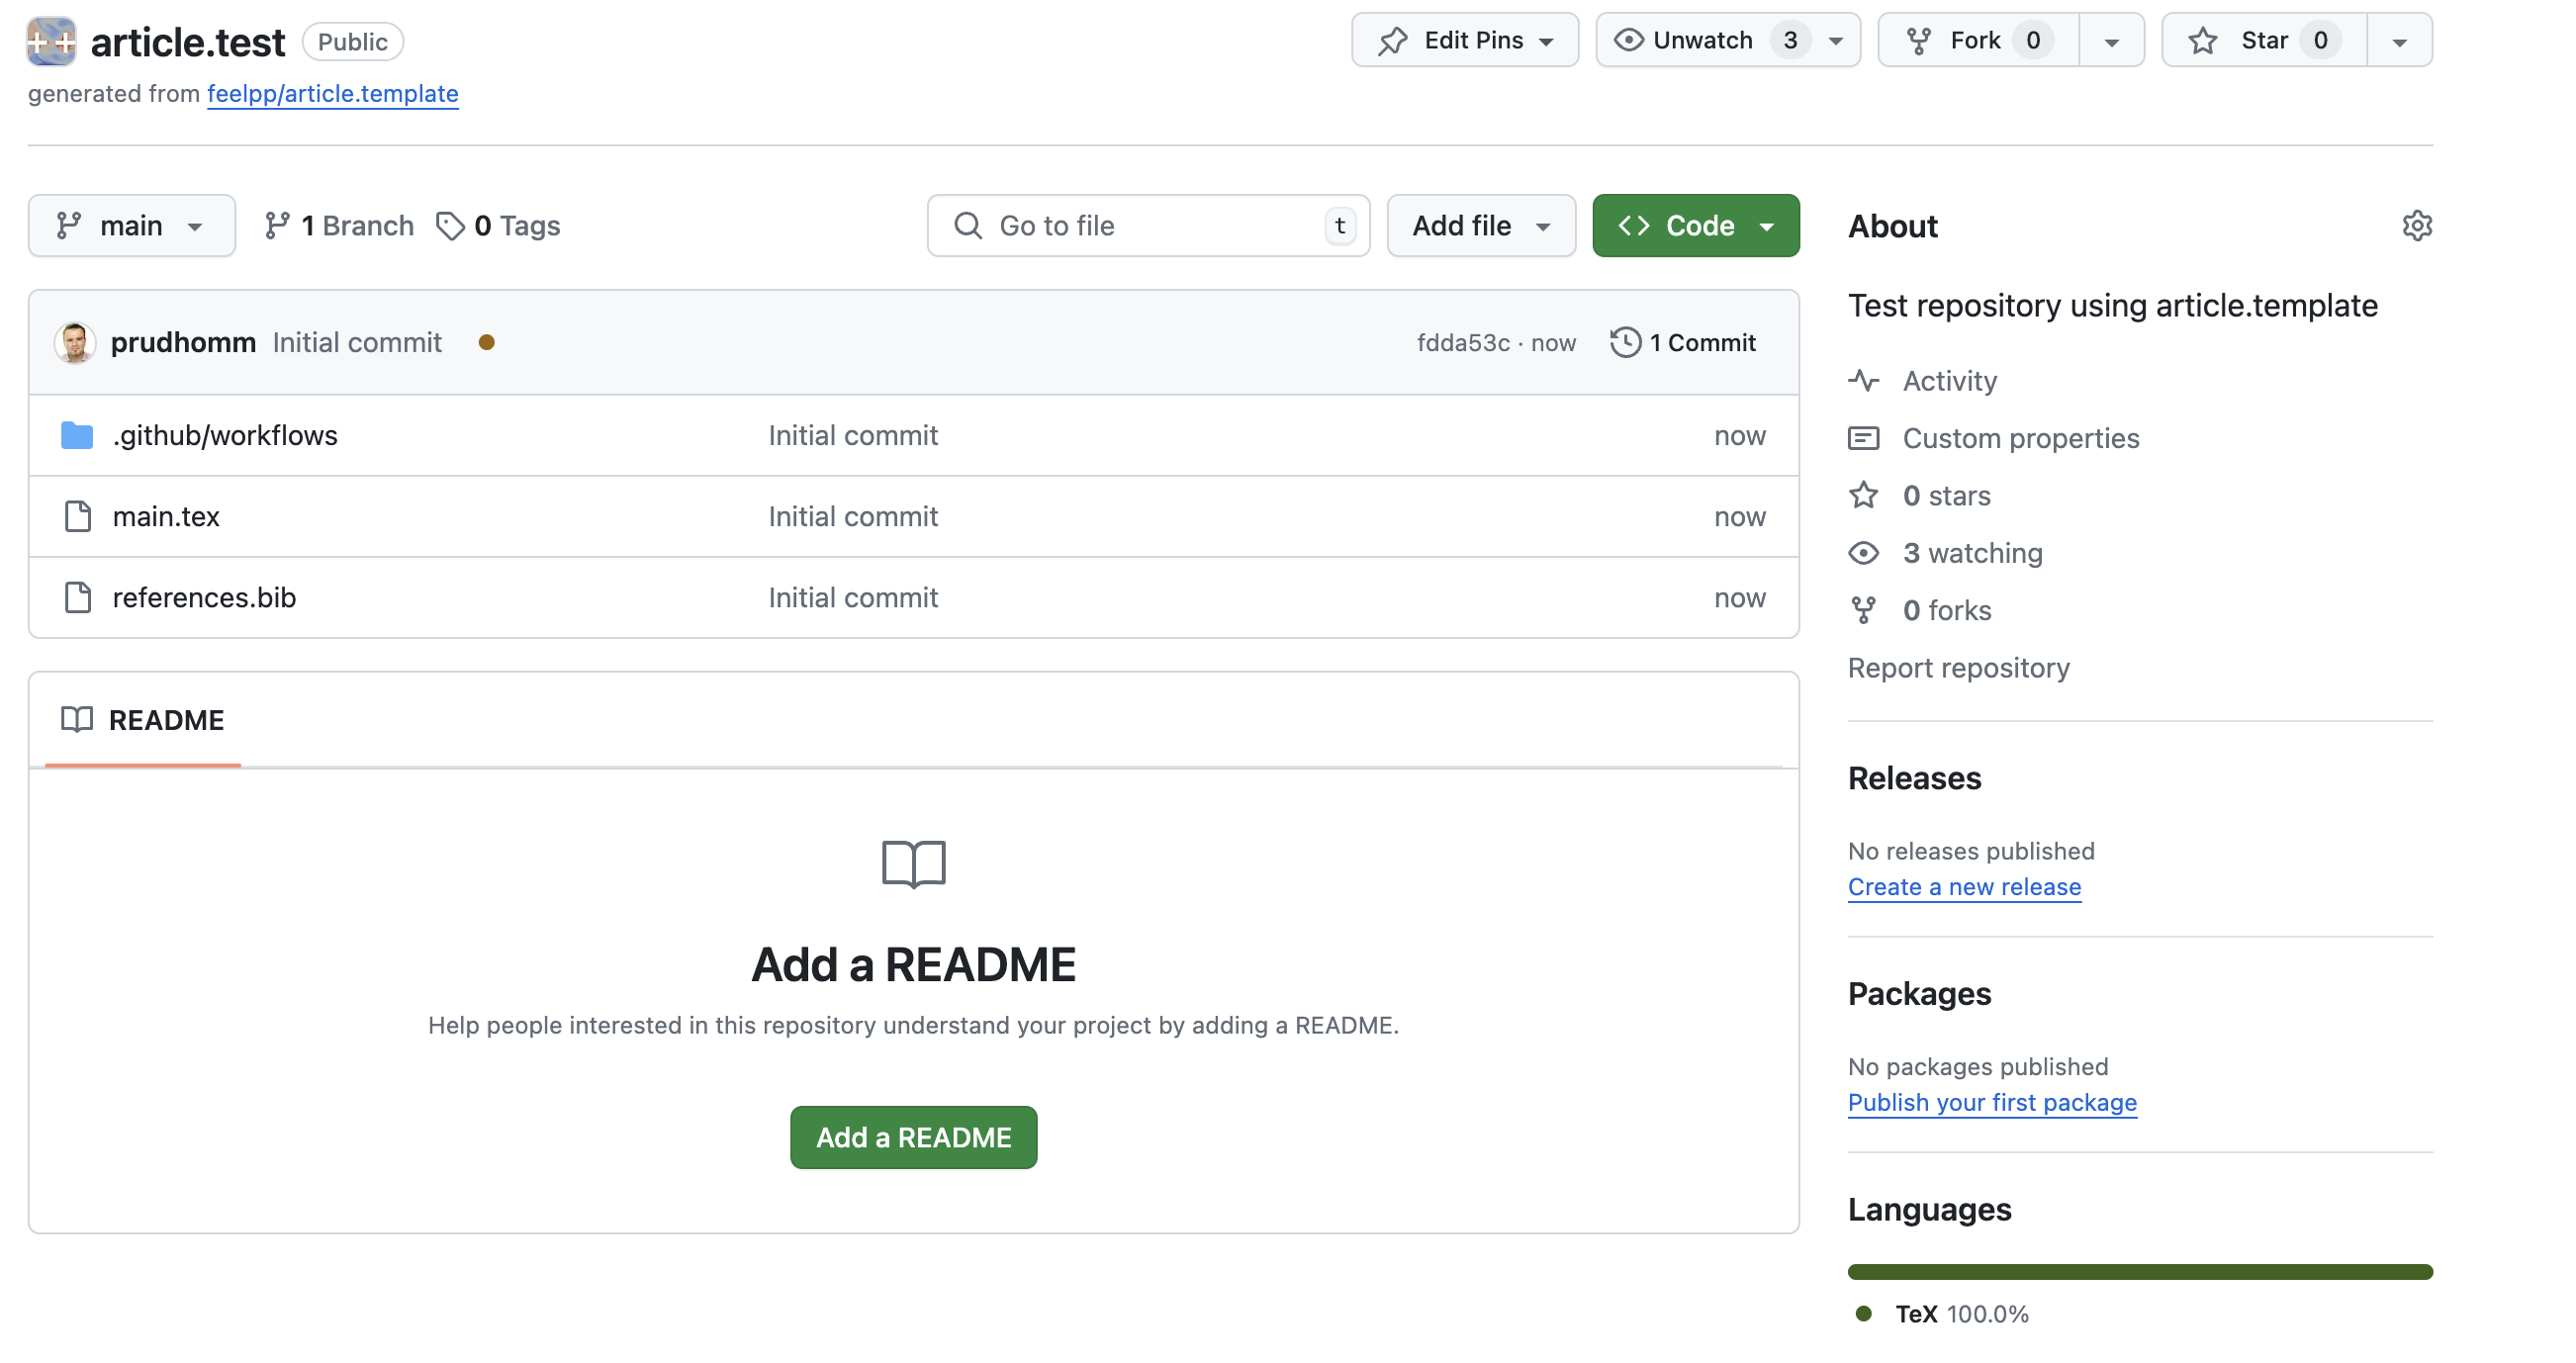
\includegraphics[width=0.8\textwidth]{img-repo-test.png}
\caption{Clone the Repository}
\end{figure}

\subsection{Add Your LaTeX Source Files}
Place your \texttt{.tex} file and image files (\texttt{img-*.pdf}, \texttt{img-*.png}, \texttt{img-*.jpg}) in the repository.

\subsection{Commit and Push Changes}
Commit your changes and push them to the repository.

\begin{minted}[bgcolor=background]{bash}
git add .
git commit -m "Add initial LaTeX document and images"
git push origin main
\end{minted}

The GitHub Action workflow will automatically compile your LaTeX document and upload the resulting PDF as an artifact. You can download the compiled PDF from the Actions tab in your repository.

\section{Overleaf Integration}

\subsection{Sync GitHub Repository with Overleaf}
\begin{enumerate}
    \item In Overleaf, create a new project and select \texttt{Import from GitHub}.
    \item Connect your GitHub account and select the repository you want to sync.
    \item The sync will trigger the workflow and compile your LaTeX document in GitHub.
\end{enumerate}

\subsection{Update References from Zotero}
\begin{enumerate}
    \item Periodically export your references from Zotero to \texttt{references.bib} and push the updated file to your GitHub repository.
    \item Overleaf will automatically sync the changes, ensuring your references are up to date.
\end{enumerate}

\section{Conclusion}
\label{sec:conclusion}

This template provides a comprehensive approach for creating and managing LaTeX articles, integrating modern tools and workflow to enhance productivity and collaboration. 
By leveraging GitHub Actions for automated compilation, Zotero for reference management, Overleaf for online editing, and Vscode using \LaTeX workshop extension for editing, researchers can streamline the writing process and focus more on content creation. 
The structured setup ensures consistent formatting and efficient handling of images and references, making it suitable for both individual use and collaborative projects.


\bibliographystyle{plainnat}
\bibliography{references}
\end{document}